\documentclass[tikz,border=12pt]{standalone}
\usepackage{tikz}
\usetikzlibrary{shapes.geometric, arrows.meta, positioning, calc, fit, backgrounds, decorations.pathreplacing}
\usepackage{amsmath,amssymb}

\begin{document}

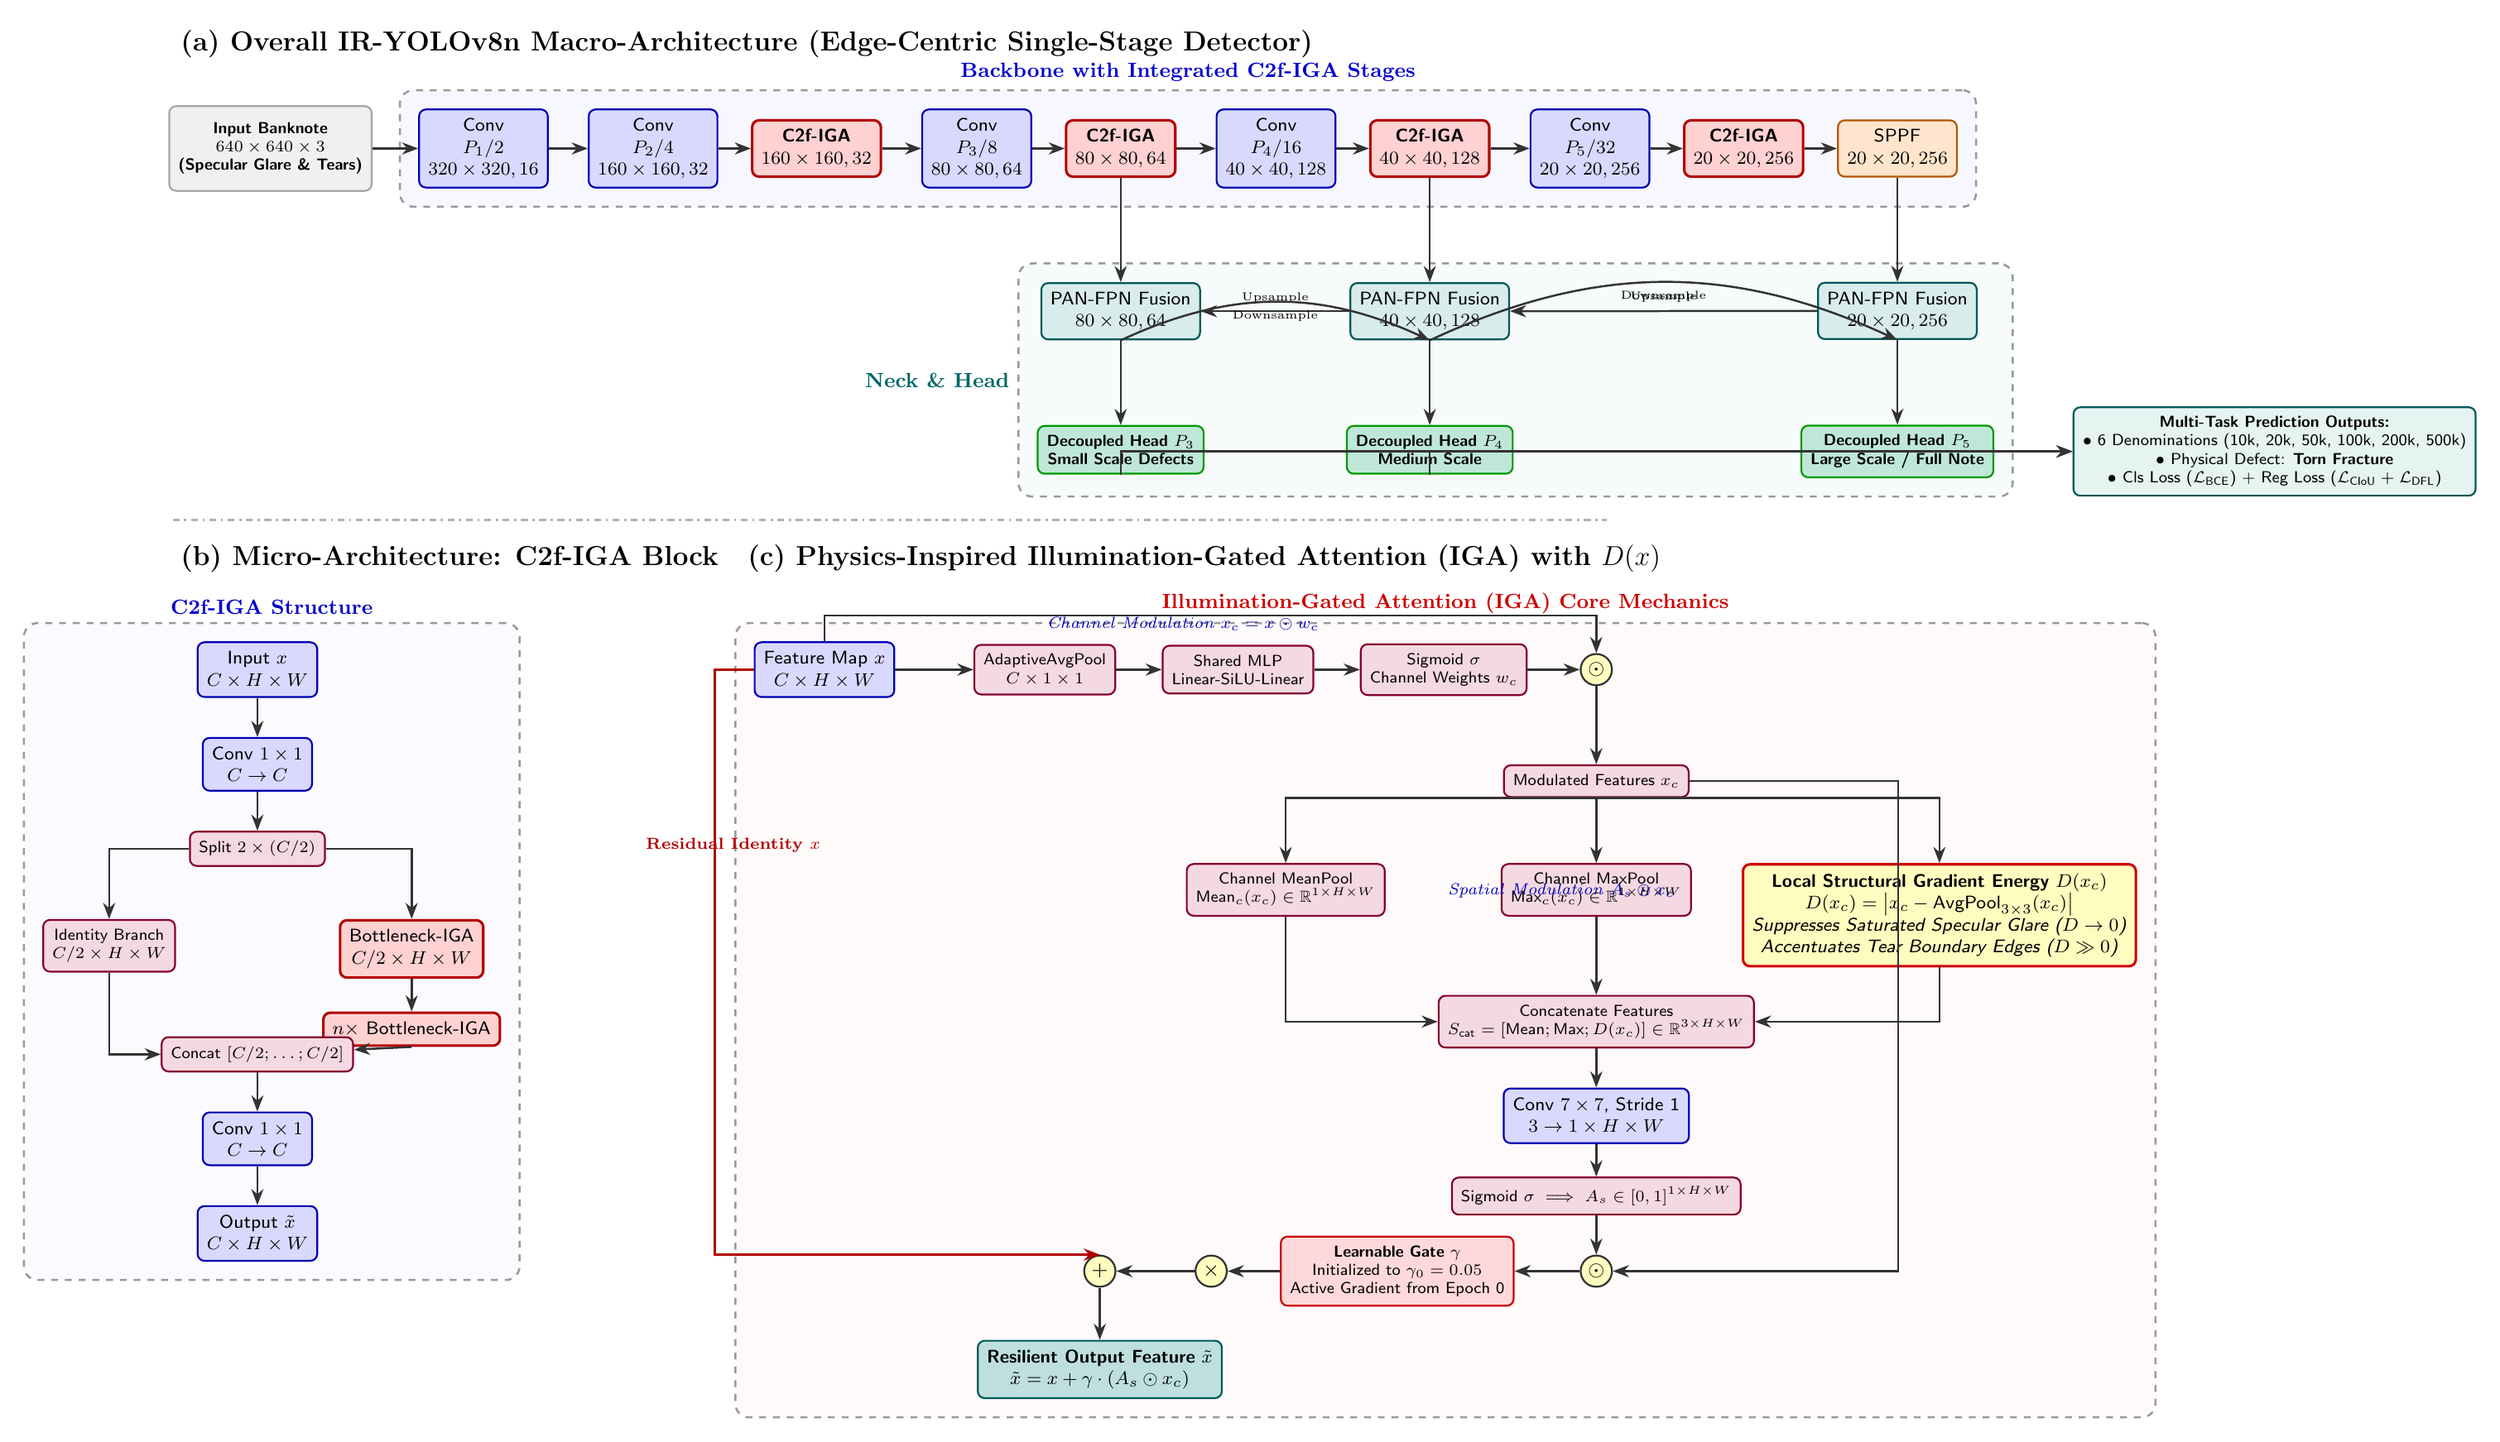
\begin{tikzpicture}[
    font=\sffamily\footnotesize,
    >=Stealth,
    node distance=0.8cm and 0.9cm,
    % Box styles
    basebox/.style={draw, rounded corners=3pt, align=center, inner sep=4pt, line width=0.8pt},
    inputbox/.style={basebox, fill=gray!12, draw=gray!70, font=\sffamily\scriptsize\bfseries},
    convbox/.style={basebox, fill=blue!15, draw=blue!70!black},
    igabox/.style={basebox, fill=red!18, draw=red!70!black, line width=1.1pt},
    sppfbox/.style={basebox, fill=orange!20, draw=orange!70!black},
    neckbox/.style={basebox, fill=teal!15, draw=teal!70!black},
    headbox/.style={basebox, fill=green!25!teal!25, draw=green!60!black, font=\sffamily\scriptsize\bfseries},
    mathbox/.style={basebox, fill=purple!15, draw=purple!70!black, font=\sffamily\scriptsize},
    opbox/.style={circle, draw=black!80, fill=yellow!25, inner sep=1.5pt, font=\bfseries\small, line width=0.8pt},
    % Arrow styles
    arrow/.style={->, line width=0.9pt, draw=black!80},
    skiparrow/.style={->, line width=0.8pt, draw=blue!60!black, dashed},
    resarrow/.style={->, line width=0.9pt, draw=red!70!black},
    % Group boxes
    groupbox/.style={draw=black!40, rounded corners=6pt, inner sep=8pt, line width=0.9pt, dashed}
]

% ==============================================================================
% TOP PANEL: PART (a) MACRO-ARCHITECTURE OF IR-YOLOv8n
% ==============================================================================
\node[font=\large\bfseries, anchor=west] (titleA) at (-1.5, 7.8) {\textbf{(a) Overall IR-YOLOv8n Macro-Architecture (Edge-Centric Single-Stage Detector)}};

% Input Image
\node[inputbox, minimum width=2.2cm, minimum height=1.3cm] (img) at (0, 6.2) {Input Banknote\\$640 \times 640 \times 3$\\(Specular Glare \& Tears)};

% Backbone Stages
\node[convbox, right=0.7cm of img] (b0) {Conv\\$P_1/2$\\$320\times 320, 16$};
\node[convbox, right=0.6cm of b0] (b1_c) {Conv\\$P_2/4$\\$160\times 160, 32$};
\node[igabox, right=0.5cm of b1_c] (b1_iga) {\textbf{C2f-IGA}\\$160\times 160, 32$};

\node[convbox, right=0.6cm of b1_iga] (b2_c) {Conv\\$P_3/8$\\$80\times 80, 64$};
\node[igabox, right=0.5cm of b2_c] (b2_iga) {\textbf{C2f-IGA}\\$80\times 80, 64$};

\node[convbox, right=0.6cm of b2_iga] (b3_c) {Conv\\$P_4/16$\\$40\times 40, 128$};
\node[igabox, right=0.5cm of b3_c] (b3_iga) {\textbf{C2f-IGA}\\$40\times 40, 128$};

\node[convbox, right=0.6cm of b3_iga] (b4_c) {Conv\\$P_5/32$\\$20\times 20, 256$};
\node[igabox, right=0.5cm of b4_c] (b4_iga) {\textbf{C2f-IGA}\\$20\times 20, 256$};
\node[sppfbox, right=0.5cm of b4_iga] (sppf) {SPPF\\$20\times 20, 256$};

% Arrows in Backbone
\draw[arrow] (img) -- (b0);
\draw[arrow] (b0) -- (b1_c);
\draw[arrow] (b1_c) -- (b1_iga);
\draw[arrow] (b1_iga) -- (b2_c);
\draw[arrow] (b2_c) -- (b2_iga);
\draw[arrow] (b2_iga) -- (b3_c);
\draw[arrow] (b3_c) -- (b3_iga);
\draw[arrow] (b3_iga) -- (b4_c);
\draw[arrow] (b4_c) -- (b4_iga);
\draw[arrow] (b4_iga) -- (sppf);

% Neck Feature Fusion Nodes (PAN-FPN)
\node[neckbox, below=1.6cm of b3_iga] (n_p4) {PAN-FPN Fusion\\$40\times 40, 128$};
\node[neckbox, below=1.6cm of b2_iga] (n_p3) {PAN-FPN Fusion\\$80\times 80, 64$};
\node[neckbox, below=1.6cm of sppf] (n_p5) {PAN-FPN Fusion\\$20\times 20, 256$};

% Connections from Backbone to Neck
\draw[arrow] (sppf.south) -- (n_p5.north);
\draw[arrow] (b3_iga.south) -- (n_p4.north);
\draw[arrow] (b2_iga.south) -- (n_p3.north);

% Lateral arrows in Neck
\draw[arrow] (n_p5) -- node[above, font=\tiny]{Upsample} (n_p4);
\draw[arrow] (n_p4) -- node[above, font=\tiny]{Upsample} (n_p3);
\draw[arrow, bend left=25] (n_p3.south) to node[below, font=\tiny]{Downsample} (n_p4.south);
\draw[arrow, bend left=25] (n_p4.south) to node[below, font=\tiny]{Downsample} (n_p5.south);

% Decoupled Detect Heads
\node[headbox, below=1.3cm of n_p3] (h_p3) {Decoupled Head $P_3$\\Small Scale Defects};
\node[headbox, below=1.3cm of n_p4] (h_p4) {Decoupled Head $P_4$\\Medium Scale};
\node[headbox, below=1.3cm of n_p5] (h_p5) {Decoupled Head $P_5$\\Large Scale / Full Note};

\draw[arrow] (n_p3) -- (h_p3);
\draw[arrow] (n_p4) -- (h_p4);
\draw[arrow] (n_p5) -- (h_p5);

% Final Output Prediction Box
\node[mathbox, right=1.2cm of h_p5, align=center, fill=green!10!teal!10, draw=teal!70!black] (out_box) {
    \textbf{Multi-Task Prediction Outputs:}\\
    $\bullet$ 6 Denominations (10k, 20k, 50k, 100k, 200k, 500k)\\
    $\bullet$ Physical Defect: \textbf{Torn Fracture}\\
    $\bullet$ Cls Loss ($\mathcal{L}_{\text{BCE}}$) + Reg Loss ($\mathcal{L}_{\text{CIoU}} + \mathcal{L}_{\text{DFL}}$)
};
\draw[arrow] (h_p5.east) -- (out_box.west);
\draw[arrow] (h_p4.south) |- (out_box.west);
\draw[arrow] (h_p3.south) |- (out_box.west);

% Backbone Group Enclosing Box
\begin{scope}[on background layer]
    \node[groupbox, fill=blue!3, fit=(b0) (sppf) (b4_iga), label={[font=\bfseries\small, text=blue!80!black]above:Backbone with Integrated C2f-IGA Stages}] (backbone_grp) {};
    \node[groupbox, fill=teal!3, fit=(n_p3) (n_p5) (h_p3) (h_p5), label={[font=\bfseries\small, text=teal!80!black]left:Neck \& Head}] (neck_grp) {};
\end{scope}

% ==============================================================================
% BOTTOM PANEL: PART (b) & (c) MICRO-ARCHITECTURE (C2f-IGA & IGA MODULE)
% ==============================================================================
\coordinate (sep) at (-1.5, 0.4);
\draw[line width=1.0pt, dash dot, draw=gray!60] (-1.5, 0.5) -- (20.5, 0.5);

\node[font=\large\bfseries, anchor=west] (titleB) at (-1.5, -0.1) {\textbf{(b) Micro-Architecture: C2f-IGA Block}};
\node[font=\large\bfseries, anchor=west] (titleC) at (7.2, -0.1) {\textbf{(c) Physics-Inspired Illumination-Gated Attention (IGA) with $D(x)$}};

% --- SUBFIGURE (b): C2f-IGA BLOCK ---
\node[convbox] (c2f_in) at (-0.2, -1.8) {Input $x$\\$C \times H \times W$};
\node[convbox, below=0.6cm of c2f_in] (c2f_conv1) {Conv $1\times 1$\\$C \to C$};
\node[mathbox, below=0.6cm of c2f_conv1] (c2f_split) {Split $2 \times (C/2)$};

\node[mathbox, below left=0.8cm and 0.2cm of c2f_split] (c2f_b1) {Identity Branch\\$C/2 \times H \times W$};
\node[igabox, below right=0.8cm and 0.2cm of c2f_split] (c2f_b2) {Bottleneck-IGA\\$C/2 \times H \times W$};
\node[igabox, below=0.5cm of c2f_b2] (c2f_b2_n) {$n \times$ Bottleneck-IGA};

\node[mathbox, below=2.6cm of c2f_split] (c2f_concat) {Concat $[C/2; \dots; C/2]$};
\node[convbox, below=0.6cm of c2f_concat] (c2f_conv2) {Conv $1\times 1$\\$C \to C$};
\node[convbox, below=0.6cm of c2f_conv2] (c2f_out) {Output $\tilde{x}$\\$C \times H \times W$};

\draw[arrow] (c2f_in) -- (c2f_conv1);
\draw[arrow] (c2f_conv1) -- (c2f_split);
\draw[arrow] (c2f_split) -| (c2f_b1.north);
\draw[arrow] (c2f_split) -| (c2f_b2.north);
\draw[arrow] (c2f_b2) -- (c2f_b2_n);
\draw[arrow] (c2f_b1.south) |- (c2f_concat.west);
\draw[arrow] (c2f_b2_n.south) -- (c2f_concat);
\draw[arrow] (c2f_concat) -- (c2f_conv2);
\draw[arrow] (c2f_conv2) -- (c2f_out);

% --- SUBFIGURE (c): IGA MODULE DETAIL ---
\node[convbox] (iga_in) at (8.5, -1.8) {Feature Map $x$\\$C \times H \times W$};

% Channel Attention Branch
\node[mathbox, right=1.2cm of iga_in] (gap) {AdaptiveAvgPool\\$C \times 1 \times 1$};
\node[mathbox, right=0.7cm of gap] (mlp) {Shared MLP\\Linear-SiLU-Linear};
\node[mathbox, right=0.7cm of mlp] (sig_c) {Sigmoid $\sigma$\\Channel Weights $w_c$};
\node[opbox, right=0.8cm of sig_c] (prod_c) {$\odot$};

\draw[arrow] (iga_in) -- (gap);
\draw[arrow] (gap) -- (mlp);
\draw[arrow] (mlp) -- (sig_c);
\draw[arrow] (sig_c) -- (prod_c);
\draw[arrow] (iga_in.north) -- ++(0, 0.4) -| (prod_c.north);
\node[font=\scriptsize\itshape, text=blue!70!black] at (14.0, -1.1) {Channel Modulation $x_c = x \odot w_c$};

% Spatial Attention Branch with D(x)
\coordinate (split_sp) at (17.5, -3.0);
\node[mathbox, below=1.2cm of prod_c] (xc_node) {Modulated Features $x_c$};
\draw[arrow] (prod_c) -- (xc_node);

% 3 Parallel Pooling Operations
\node[mathbox, below left=1.0cm and 1.8cm of xc_node] (sp_mean) {Channel MeanPool\\$\text{Mean}_c(x_c) \in \mathbb{R}^{1 \times H \times W}$};
\node[mathbox, below=1.0cm of xc_node] (sp_max) {Channel MaxPool\\$\text{Max}_c(x_c) \in \mathbb{R}^{1 \times H \times W}$};
\node[igabox, fill=yellow!25, draw=red!80!black, below right=1.0cm and 0.8cm of xc_node] (sp_grad) {
    \textbf{Local Structural Gradient Energy $D(x_c)$}\\
    $D(x_c) = \left| x_c - \text{AvgPool}_{3\times 3}(x_c) \right|$\\
    \textit{Suppresses Saturated Specular Glare ($D \to 0$)}\\
    \textit{Accentuates Tear Boundary Edges ($D \gg 0$)}
};

\draw[arrow] (xc_node.south) -| (sp_mean.north);
\draw[arrow] (xc_node.south) -- (sp_max.north);
\draw[arrow] (xc_node.south) -| (sp_grad.north);

% Concatenate 3 maps
\node[mathbox, below=1.2cm of sp_max] (sp_concat) {Concatenate Features\\$S_{\text{cat}} = [\text{Mean}; \text{Max}; D(x_c)] \in \mathbb{R}^{3 \times H \times W}$};
\draw[arrow] (sp_mean.south) |- (sp_concat.west);
\draw[arrow] (sp_max.south) -- (sp_concat);
\draw[arrow] (sp_grad.south) |- (sp_concat.east);

% Conv 7x7 and Sigmoid
\node[convbox, below=0.6cm of sp_concat] (conv7) {Conv $7 \times 7$, Stride 1\\$3 \to 1 \times H \times W$};
\node[mathbox, below=0.5cm of conv7] (sig_s) {Sigmoid $\sigma \implies A_s \in [0, 1]^{1 \times H \times W}$};
\node[opbox, below=0.6cm of sig_s] (prod_s) {$\odot$};

\draw[arrow] (sp_concat) -- (conv7);
\draw[arrow] (conv7) -- (sig_s);
\draw[arrow] (sig_s) -- (prod_s);

% Modulate xc with As
\draw[arrow] (xc_node.east) -- ++(3.2, 0) |- (prod_s.east);
\node[font=\scriptsize\itshape, text=blue!70!black] at (19.8, -5.2) {Spatial Modulation $A_s \odot x_c$};

% Learnable Gating Scale gamma
\node[mathbox, fill=red!15, draw=red!80!black, left=1.0cm of prod_s] (gamma_node) {
    \textbf{Learnable Gate} $\gamma$\\
    Initialized to $\gamma_0 = 0.05$\\
    Active Gradient from Epoch 0
};
\node[opbox, left=0.8cm of gamma_node] (prod_gamma) {$\times$};
\draw[arrow] (prod_s) -- (gamma_node);
\draw[arrow] (gamma_node) -- (prod_gamma);

% Final Residual Add
\node[opbox, left=1.2cm of prod_gamma] (res_add) {$+$};
\draw[arrow] (prod_gamma) -- (res_add);

% Residual skip from input x
\draw[resarrow] (iga_in.west) -- ++(-0.6, 0) |- (res_add.north);
\node[font=\scriptsize\bfseries, text=red!70!black] at (7.1, -4.5) {Residual Identity $x$};

% Output node
\node[convbox, fill=teal!25, draw=teal!70!black, below=0.8cm of res_add] (iga_out) {
    \textbf{Resilient Output Feature} $\tilde{x}$\\
    $\tilde{x} = x + \gamma \cdot (A_s \odot x_c)$
};
\draw[arrow] (res_add) -- (iga_out);

% Surrounding group for IGA
\begin{scope}[on background layer]
    \node[groupbox, fill=red!2, fit=(iga_in) (gap) (sig_c) (sp_grad) (prod_s) (res_add) (iga_out), label={[font=\bfseries\small, text=red!80!black]above:Illumination-Gated Attention (IGA) Core Mechanics}] (iga_grp) {};
    \node[groupbox, fill=blue!2, fit=(c2f_in) (c2f_out) (c2f_b1) (c2f_b2_n), label={[font=\bfseries\small, text=blue!80!black]above:C2f-IGA Structure}] (c2f_grp) {};
\end{scope}

\end{tikzpicture}
\end{document}
